%% Options for packages loaded elsewhere
%% Options for packages loaded elsewhere
%\PassOptionsToPackage{unicode}{hyperref}
%\PassOptionsToPackage{hyphens}{url}
%\PassOptionsToPackage{dvipsnames,svgnames,x11names}{xcolor}
%%
%\documentclass[
%]{IEEEtran}
%\usepackage{xcolor}
%\usepackage{amsmath,amssymb}
%\setcounter{secnumdepth}{5}
%\usepackage{iftex}
%\ifPDFTeX
%  \usepackage[T1]{fontenc}
%  \usepackage[utf8]{inputenc}
%  \usepackage{textcomp} % provide euro and other symbols
%\else % if luatex or xetex
%  \usepackage{unicode-math} % this also loads fontspec
%  \defaultfontfeatures{Scale=MatchLowercase}
%  \defaultfontfeatures[\rmfamily]{Ligatures=TeX,Scale=1}
%\fi
%\usepackage{lmodern}
%\ifPDFTeX\else
%  % xetex/luatex font selection
%\fi
%% Use upquote if available, for straight quotes in verbatim environments
%\IfFileExists{upquote.sty}{\usepackage{upquote}}{}
%\IfFileExists{microtype.sty}{% use microtype if available
%  \usepackage[]{microtype}
%  \UseMicrotypeSet[protrusion]{basicmath} % disable protrusion for tt fonts
%}{}
%\makeatletter
%\@ifundefined{KOMAClassName}{% if non-KOMA class
%  \IfFileExists{parskip.sty}{%
%    \usepackage{parskip}
%  }{% else
%    \setlength{\parindent}{0pt}
%    \setlength{\parskip}{6pt plus 2pt minus 1pt}}
%}{% if KOMA class
%  \KOMAoptions{parskip=half}}
%\makeatother
%% Make \paragraph and \subparagraph free-standing
%\makeatletter
%\ifx\paragraph\undefined\else
%  \let\oldparagraph\paragraph
%  \renewcommand{\paragraph}{
%    \@ifstar
%      \xxxParagraphStar
%      \xxxParagraphNoStar
%  }
%  \newcommand{\xxxParagraphStar}[1]{\oldparagraph*{#1}\mbox{}}
%  \newcommand{\xxxParagraphNoStar}[1]{\oldparagraph{#1}\mbox{}}
%\fi
%\ifx\subparagraph\undefined\else
%  \let\oldsubparagraph\subparagraph
%  \renewcommand{\subparagraph}{
%    \@ifstar
%      \xxxSubParagraphStar
%      \xxxSubParagraphNoStar
%  }
%  \newcommand{\xxxSubParagraphStar}[1]{\oldsubparagraph*{#1}\mbox{}}
%  \newcommand{\xxxSubParagraphNoStar}[1]{\oldsubparagraph{#1}\mbox{}}
%\fi
%\makeatother
%
%\usepackage{color}
%\usepackage{fancyvrb}
%\newcommand{\VerbBar}{|}
%\newcommand{\VERB}{\Verb[commandchars=\\\{\}]}
%\DefineVerbatimEnvironment{Highlighting}{Verbatim}{commandchars=\\\{\}}
%% Add ',fontsize=\small' for more characters per line
%\usepackage{framed}
%\definecolor{shadecolor}{RGB}{241,243,245}
%\newenvironment{Shaded}{\begin{snugshade}}{\end{snugshade}}
%\newcommand{\AlertTok}[1]{\textcolor[rgb]{0.68,0.00,0.00}{#1}}
%\newcommand{\AnnotationTok}[1]{\textcolor[rgb]{0.37,0.37,0.37}{#1}}
%\newcommand{\AttributeTok}[1]{\textcolor[rgb]{0.40,0.45,0.13}{#1}}
%\newcommand{\BaseNTok}[1]{\textcolor[rgb]{0.68,0.00,0.00}{#1}}
%\newcommand{\BuiltInTok}[1]{\textcolor[rgb]{0.00,0.23,0.31}{#1}}
%\newcommand{\CharTok}[1]{\textcolor[rgb]{0.13,0.47,0.30}{#1}}
%\newcommand{\CommentTok}[1]{\textcolor[rgb]{0.37,0.37,0.37}{#1}}
%\newcommand{\CommentVarTok}[1]{\textcolor[rgb]{0.37,0.37,0.37}{\textit{#1}}}
%\newcommand{\ConstantTok}[1]{\textcolor[rgb]{0.56,0.35,0.01}{#1}}
%\newcommand{\ControlFlowTok}[1]{\textcolor[rgb]{0.00,0.23,0.31}{\textbf{#1}}}
%\newcommand{\DataTypeTok}[1]{\textcolor[rgb]{0.68,0.00,0.00}{#1}}
%\newcommand{\DecValTok}[1]{\textcolor[rgb]{0.68,0.00,0.00}{#1}}
%\newcommand{\DocumentationTok}[1]{\textcolor[rgb]{0.37,0.37,0.37}{\textit{#1}}}
%\newcommand{\ErrorTok}[1]{\textcolor[rgb]{0.68,0.00,0.00}{#1}}
%\newcommand{\ExtensionTok}[1]{\textcolor[rgb]{0.00,0.23,0.31}{#1}}
%\newcommand{\FloatTok}[1]{\textcolor[rgb]{0.68,0.00,0.00}{#1}}
%\newcommand{\FunctionTok}[1]{\textcolor[rgb]{0.28,0.35,0.67}{#1}}
%\newcommand{\ImportTok}[1]{\textcolor[rgb]{0.00,0.46,0.62}{#1}}
%\newcommand{\InformationTok}[1]{\textcolor[rgb]{0.37,0.37,0.37}{#1}}
%\newcommand{\KeywordTok}[1]{\textcolor[rgb]{0.00,0.23,0.31}{\textbf{#1}}}
%\newcommand{\NormalTok}[1]{\textcolor[rgb]{0.00,0.23,0.31}{#1}}
%\newcommand{\OperatorTok}[1]{\textcolor[rgb]{0.37,0.37,0.37}{#1}}
%\newcommand{\OtherTok}[1]{\textcolor[rgb]{0.00,0.23,0.31}{#1}}
%\newcommand{\PreprocessorTok}[1]{\textcolor[rgb]{0.68,0.00,0.00}{#1}}
%\newcommand{\RegionMarkerTok}[1]{\textcolor[rgb]{0.00,0.23,0.31}{#1}}
%\newcommand{\SpecialCharTok}[1]{\textcolor[rgb]{0.37,0.37,0.37}{#1}}
%\newcommand{\SpecialStringTok}[1]{\textcolor[rgb]{0.13,0.47,0.30}{#1}}
%\newcommand{\StringTok}[1]{\textcolor[rgb]{0.13,0.47,0.30}{#1}}
%\newcommand{\VariableTok}[1]{\textcolor[rgb]{0.07,0.07,0.07}{#1}}
%\newcommand{\VerbatimStringTok}[1]{\textcolor[rgb]{0.13,0.47,0.30}{#1}}
%\newcommand{\WarningTok}[1]{\textcolor[rgb]{0.37,0.37,0.37}{\textit{#1}}}
%
%\usepackage{longtable,booktabs,array}
%\usepackage{calc} % for calculating minipage widths
%% Correct order of tables after \paragraph or \subparagraph
%\usepackage{etoolbox}
%\makeatletter
%\patchcmd\longtable{\par}{\if@noskipsec\mbox{}\fi\par}{}{}
%\makeatother
%% Allow footnotes in longtable head/foot
%\IfFileExists{footnotehyper.sty}{\usepackage{footnotehyper}}{\usepackage{footnote}}
%\makesavenoteenv{longtable}
%\usepackage{graphicx}
%\makeatletter
%\newsavebox\pandoc@box
%\newcommand*\pandocbounded[1]{% scales image to fit in text height/width
%  \sbox\pandoc@box{#1}%
%  \Gscale@div\@tempa{\textheight}{\dimexpr\ht\pandoc@box+\dp\pandoc@box\relax}%
%  \Gscale@div\@tempb{\linewidth}{\wd\pandoc@box}%
%  \ifdim\@tempb\p@<\@tempa\p@\let\@tempa\@tempb\fi% select the smaller of both
%  \ifdim\@tempa\p@<\p@\scalebox{\@tempa}{\usebox\pandoc@box}%
%  \else\usebox{\pandoc@box}%
%  \fi%
%}
%% Set default figure placement to htbp
%\def\fps@figure{htbp}
%\makeatother
%
%
%
%
%
%\setlength{\emergencystretch}{3em} % prevent overfull lines
%
%\providecommand{\tightlist}{%
%  \setlength{\itemsep}{0pt}\setlength{\parskip}{0pt}}
%
%
%
% 
%
%
%\makeatletter
%\@ifpackageloaded{caption}{}{\usepackage{caption}}
%\AtBeginDocument{%
%\ifdefined\contentsname
%  \renewcommand*\contentsname{Table of contents}
%\else
%  \newcommand\contentsname{Table of contents}
%\fi
%\ifdefined\listfigurename
%  \renewcommand*\listfigurename{List of Figures}
%\else
%  \newcommand\listfigurename{List of Figures}
%\fi
%\ifdefined\listtablename
%  \renewcommand*\listtablename{List of Tables}
%\else
%  \newcommand\listtablename{List of Tables}
%\fi
%\ifdefined\figurename
%  \renewcommand*\figurename{Figure}
%\else
%  \newcommand\figurename{Figure}
%\fi
%\ifdefined\tablename
%  \renewcommand*\tablename{Table}
%\else
%  \newcommand\tablename{Table}
%\fi
%}
%\@ifpackageloaded{float}{}{\usepackage{float}}
%\floatstyle{ruled}
%\@ifundefined{c@chapter}{\newfloat{codelisting}{h}{lop}}{\newfloat{codelisting}{h}{lop}[chapter]}
%\floatname{codelisting}{Listing}
%\newcommand*\listoflistings{\listof{codelisting}{List of Listings}}
%\makeatother
%\makeatletter
%\makeatother
%\makeatletter
%\@ifpackageloaded{caption}{}{\usepackage{caption}}
%\@ifpackageloaded{subcaption}{}{\usepackage{subcaption}}
%\makeatother
%\usepackage{bookmark}
%\IfFileExists{xurl.sty}{\usepackage{xurl}}{} % add URL line breaks if available
%\urlstyle{same}
%\hypersetup{
%  pdftitle={Perceptron implementation},
%  colorlinks=true,
%  linkcolor={blue},
%  filecolor={Maroon},
%  citecolor={Blue},
%  urlcolor={Blue},
%  pdfcreator={LaTeX via pandoc}}
%
%
%\title{Perceptron implementation}
%\author{}
%\date{}
%\begin{document}
%\maketitle


\section{Perceptron algorithm
implementation}\label{perceptron-algorithm-implementation}

I'll use numpy as a very common package used for scientific computation,
\textbf{make\_blobs} from Sci-kit learn for data generation and pyplot
from matplotlib for data visualization.

\begin{Shaded}
\begin{Highlighting}[]
\CommentTok{\#!pip install scikit{-}learn}
\ImportTok{import}\NormalTok{ numpy }\ImportTok{as}\NormalTok{ np}
\ImportTok{from}\NormalTok{ sklearn.datasets }\ImportTok{import}\NormalTok{ make\_blobs}
\ImportTok{import}\NormalTok{ matplotlib.pyplot }\ImportTok{as}\NormalTok{ plt}
\end{Highlighting}
\end{Shaded}

Now, in order to implement a perceptron we have to define the three
steps needed and the evaluation function

\subsection{Neuron Model}\label{neuron-model}

First the perceptron output, which is the most important element, it's
the neuron model. It will receive a vector of inputs \(X_{jk}\) a vector
of weights \(W_{jk}\) and a reference for the activation function
\(S(\cdot)\).

\begin{Shaded}
\begin{Highlighting}[]
\KeywordTok{def}\NormalTok{ perceptronOutput(W,X,bias,ActivationFunction):}
\NormalTok{  WeighedInputs }\OperatorTok{=}\NormalTok{ np.dot(W,X)}
\NormalTok{  Net }\OperatorTok{=}\NormalTok{ WeighedInputs }\OperatorTok{{-}}\NormalTok{ bias}
\NormalTok{  O }\OperatorTok{=}\NormalTok{ ActivationFunction(Net)}
  \ControlFlowTok{return}\NormalTok{ O}
\end{Highlighting}
\end{Shaded}

\subsection{Error equation}\label{error-equation}

This function computes the error of the perceptron based on its output
compared to the desired output. It receives the perceptron output vector
\(O_j\), the desired output vector \(Y_j\) and the number of patterns
\(N\).

\begin{Shaded}
\begin{Highlighting}[]
\KeywordTok{def}\NormalTok{ computeError(Y,O,N):}
\NormalTok{  DeltaSum }\OperatorTok{=}\NormalTok{ np.}\BuiltInTok{sum}\NormalTok{(np.}\BuiltInTok{abs}\NormalTok{(Y}\OperatorTok{{-}}\NormalTok{O))}
\NormalTok{  Err }\OperatorTok{=}\NormalTok{ DeltaSum}\OperatorTok{/}\NormalTok{N}
  \ControlFlowTok{return}\NormalTok{ Err}
\end{Highlighting}
\end{Shaded}

\subsection{Weights update function}\label{weights-update-function}

This function receives the current weights vector \(W_j\), the
perceptron and desired output vectors \(O_j\) and \(Y_j\) and learning
rate \(r\). Then returns the new weights vector.

\begin{Shaded}
\begin{Highlighting}[]
\KeywordTok{def}\NormalTok{ updateWeights(Y,O,W,X,r):}
\NormalTok{  NewWeights }\OperatorTok{=}\NormalTok{ W }\OperatorTok{{-}}\NormalTok{ (Y}\OperatorTok{{-}}\NormalTok{O)}\OperatorTok{*}\NormalTok{X}\OperatorTok{*}\NormalTok{r}
  \ControlFlowTok{return}\NormalTok{  NewWeights}
\end{Highlighting}
\end{Shaded}

\subsection{Evaluation function}\label{evaluation-function}

For this one, I'll create my own evaluation function based on a
normalized {[}0,1{]} sign function.

\(S(X) = \begin{cases}
  1, &X >     0\\
  0, &X \leq  0\\
\end{cases}\)

\begin{Shaded}
\begin{Highlighting}[]
\KeywordTok{def}\NormalTok{ S(Net):}
  \ControlFlowTok{if}\NormalTok{ Net}\OperatorTok{\textless{}}\DecValTok{1}\NormalTok{ :}
    \ControlFlowTok{return} \DecValTok{0}\OperatorTok{;}
  \ControlFlowTok{return} \DecValTok{1}\OperatorTok{;}
\end{Highlighting}
\end{Shaded}

\section{Training}\label{training}

\subsection{Input data}\label{input-data}

Using Scikit-Learn I'll create a new dataset of inputs and its desired
output (classification) in order to train our perceptron.

\begin{Shaded}
\begin{Highlighting}[]
\CommentTok{\# This one is to get 3000 elements to classify}
\NormalTok{N}\OperatorTok{=}\DecValTok{3000}
\CommentTok{\# Two features to input the perceptron}
\NormalTok{nFeatures}\OperatorTok{=}\DecValTok{2}
\NormalTok{X,Y }\OperatorTok{=}\NormalTok{ make\_blobs(}
  \CommentTok{\# Number of elements  \# Number of features}
\NormalTok{  n\_samples}\OperatorTok{=}\NormalTok{N,          n\_features}\OperatorTok{=}\NormalTok{nFeatures,}
  \CommentTok{\# Two classes         \# Standard deviation}
\NormalTok{  centers}\OperatorTok{=}\DecValTok{2}\NormalTok{,            cluster\_std}\OperatorTok{=}\FloatTok{1.9}\NormalTok{,}
  \CommentTok{\# Only to get randomly positioned}
\NormalTok{  shuffle}\OperatorTok{=}\VariableTok{True}\NormalTok{,}
  \CommentTok{\# Random Seed}
\NormalTok{  random\_state}\OperatorTok{=}\DecValTok{1201931}
\NormalTok{)}
\NormalTok{plt.scatter(X[:,}\DecValTok{0}\NormalTok{],X[:,}\DecValTok{1}\NormalTok{],c}\OperatorTok{=}\NormalTok{Y,cmap}\OperatorTok{=}\StringTok{\textquotesingle{}magma\textquotesingle{}}\NormalTok{,s}\OperatorTok{=}\DecValTok{5}\NormalTok{)}
\NormalTok{plt.xlabel(}\StringTok{\textquotesingle{}Feature 1\textquotesingle{}}\NormalTok{)}
\NormalTok{plt.xlabel(}\StringTok{\textquotesingle{}Feature 2\textquotesingle{}}\NormalTok{)}
\NormalTok{plt.title(}\StringTok{\textquotesingle{}Sample space\textquotesingle{}}\NormalTok{)}
\NormalTok{plt.colorbar(label}\OperatorTok{=}\StringTok{"Classes"}\NormalTok{)}
\NormalTok{plt.show()}
\end{Highlighting}
\end{Shaded}

\pandocbounded{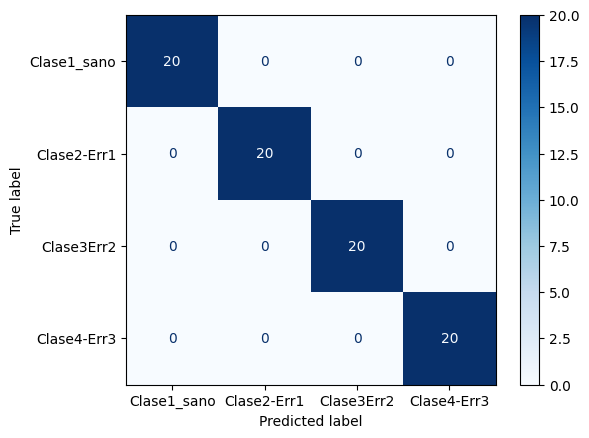
\includegraphics[keepaspectratio]{perceptron_files/figure-latex/cell-7-output-1.png}}

Then I'll derived of the features quantity, I'll create a weights vetor
\(W\). And create a function which will process a datum.

\begin{Shaded}
\begin{Highlighting}[]
\NormalTok{bias }\OperatorTok{=} \OperatorTok{{-}}\FloatTok{0.2}
\NormalTok{learnRate }\OperatorTok{=} \FloatTok{0.6}
\NormalTok{W}\OperatorTok{=}\NormalTok{np.zeros(nFeatures)}
\ControlFlowTok{for}\NormalTok{ i }\KeywordTok{in} \BuiltInTok{range}\NormalTok{(}\BuiltInTok{len}\NormalTok{(X)):}
\NormalTok{  Xi }\OperatorTok{=}\NormalTok{ X[i]}\OperatorTok{;}\NormalTok{ Yi }\OperatorTok{=}\NormalTok{ Y[i]}\OperatorTok{;}
\NormalTok{  Oi}\OperatorTok{=}\NormalTok{perceptronOutput(Xi,W,bias,S)}
\NormalTok{  Err}\OperatorTok{=}\NormalTok{computeError(Yi,Oi,N)}
\NormalTok{  W}\OperatorTok{=}\NormalTok{updateWeights(Yi,Oi,W,Xi,learnRate)}
\end{Highlighting}
\end{Shaded}

Then I'll plot the sample space with a frontier made by the weights

\begin{Shaded}
\begin{Highlighting}[]
\NormalTok{m}\OperatorTok{={-}}\NormalTok{W[}\DecValTok{0}\NormalTok{]}\OperatorTok{/}\NormalTok{W[}\DecValTok{1}\NormalTok{]}
\NormalTok{Po}\OperatorTok{=}\NormalTok{[ }\BuiltInTok{min}\NormalTok{(X[:,}\DecValTok{0}\NormalTok{]) , }\BuiltInTok{max}\NormalTok{(X[:,}\DecValTok{1}\NormalTok{]) ]}
\NormalTok{Pf}\OperatorTok{=}\NormalTok{np.multiply(Po,m)}\OperatorTok{+}\NormalTok{np.divide(bias,W[}\DecValTok{1}\NormalTok{])}

\NormalTok{plt.plot(Po,Pf,}\StringTok{\textquotesingle{}g{-}\textquotesingle{}}\NormalTok{,linewidth}\OperatorTok{=}\FloatTok{0.8}\NormalTok{)}
\NormalTok{plt.scatter(X[:,}\DecValTok{0}\NormalTok{],X[:,}\DecValTok{1}\NormalTok{],c}\OperatorTok{=}\NormalTok{Y,cmap}\OperatorTok{=}\StringTok{\textquotesingle{}magma\textquotesingle{}}\NormalTok{,s}\OperatorTok{=}\DecValTok{5}\NormalTok{)}
\NormalTok{plt.xlabel(}\StringTok{\textquotesingle{}Feature 1\textquotesingle{}}\NormalTok{)}
\NormalTok{plt.xlabel(}\StringTok{\textquotesingle{}Feature 2\textquotesingle{}}\NormalTok{)}
\NormalTok{plt.title(}\StringTok{\textquotesingle{}Sample space\textquotesingle{}}\NormalTok{)}
\NormalTok{plt.colorbar(label}\OperatorTok{=}\StringTok{"Classes"}\NormalTok{)}
\NormalTok{plt.show()}
\end{Highlighting}
\end{Shaded}

\pandocbounded{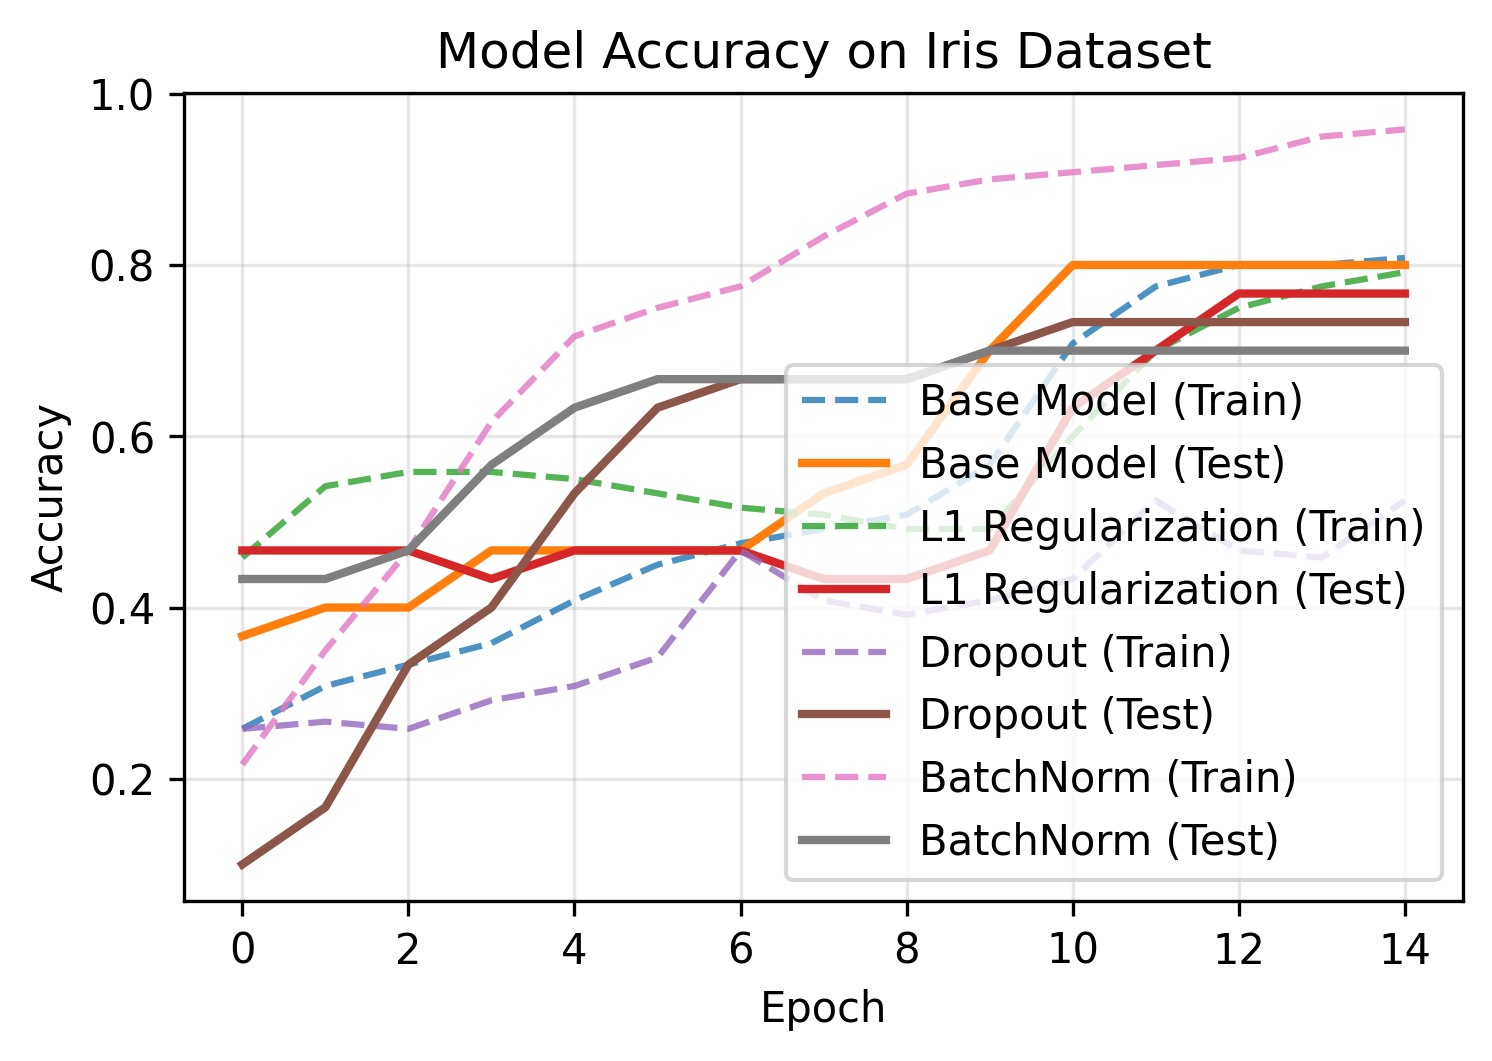
\includegraphics[keepaspectratio]{perceptron_files/figure-latex/cell-9-output-1.png}}




%\end{document}
